% !TEX root = ../main.tex

% TODO inform dietrich of the Technologies/Structure switch

\chapter{Technologies used}
\label{ch:technologiesUsed}

In this chapter, technologies used in the project and subsequently shown in code samples in later chapters will be introduced.
This enables a better understanding of the code samples and comprehension of the underlying theory.\\
Technologies like libraries and frameworks that are specific to certain methodologies,
meaning that they are or contain the implementation of said methodologies,
and are only used for that implementation,
will be explained in the respective methodologies's section of this thesis.\\
Furthermore, the technologies used for the dashboard will only be explained in the respective chapter,
since the dashboard is only used for the interaction with and visualization of the underlying analysis,
not for the analysis itself.

\section{Languages}
\label{sec:languages}

Only the Python programming language was used, since it is general-purpose,
has a high level of abstraction and focuses on readability,
which will be beneficial when working with complex architectures and algorithms later on.
Python follows multiple paradigms.
It is object-oriented, imperative, procedural and reflective~\cite{van2007python}.
It also supports dynamic typing, which enables its users to focus on higher-level tasks, at the cost of computational efficiency \cite{Perez-schofield2010}.
Since its inital release in 1991, these and more aspects have made it a popular choice among researches.
As seen in~\ref{table:python}, there are currently 2 supported versions of Python, which are not backwards compatible.
In this thesis, version 3.6.2 is used.
Furthermore, virtualenv was used to make the development environment easily reproducible on other machines.

% TODO ask dietrich how to properly cite this excerpt from van2007python, since some part are just copied over
\begin{table}
    \caption{The Python programming language~\cite{van2007python}}
    \label{table:python}
    \vspace{0.2cm}
    \begin{tabular}{l | l} %
        Paradigms
        & Multi-paradigm: object-oriented, imperative, functional,
        \\ & procedural, reflective
        \\ \midrule
        Appeared in
        & 1991
        \\ \midrule
        Designed by
        & Guido van Rossum
        % TODO properly link to his name
        \\ \midrule
        Developer
        & Python Software Foundation
        % TODO properly link to the Python software foundation
        \\ \midrule
        Stable releases
        & 3.6.2 and 2.7.13 (8. September 2017)
        \\ \midrule
        Typing discipline
        & duck, dynamic, strong
        \\ \midrule
        OS
        & cross-platform
        \\ \midrule
        Usual filename extensions
        & .py, .pyw, .pyc, .pyo, .pyd
    \end{tabular}
\end{table}

% TODO maybe also talk about other languages considered, with comparison table


\section{Libraries}
\label{sec:libraries}

\subsection{Kafka}
\label{subsec:kafka}

Kafka is a distributed messaging system implementing the publish/subscribe paradigm.
In the publish/subscribe paradigm, subscribers register their interest in a certain type of event,
and are asynchronously notified by the system when an event is published that matches the criteria~\cite{Eugster2003}.
In Kafka, the publishing entities are called producers, and the subscribing entities are called consumers.
A stream of events (called messages in Kafka) of a particular type that a consumer can subscribe to is defined by a topic~\cite{Kreps2015}.

% include diagram
\begin{figure}
    \centering
    \caption{Simplified diagram of a typical Kafka setup.}
    \label{fig:kafka}
    % TODO smaller maybe it somehow fits next to the python table.
    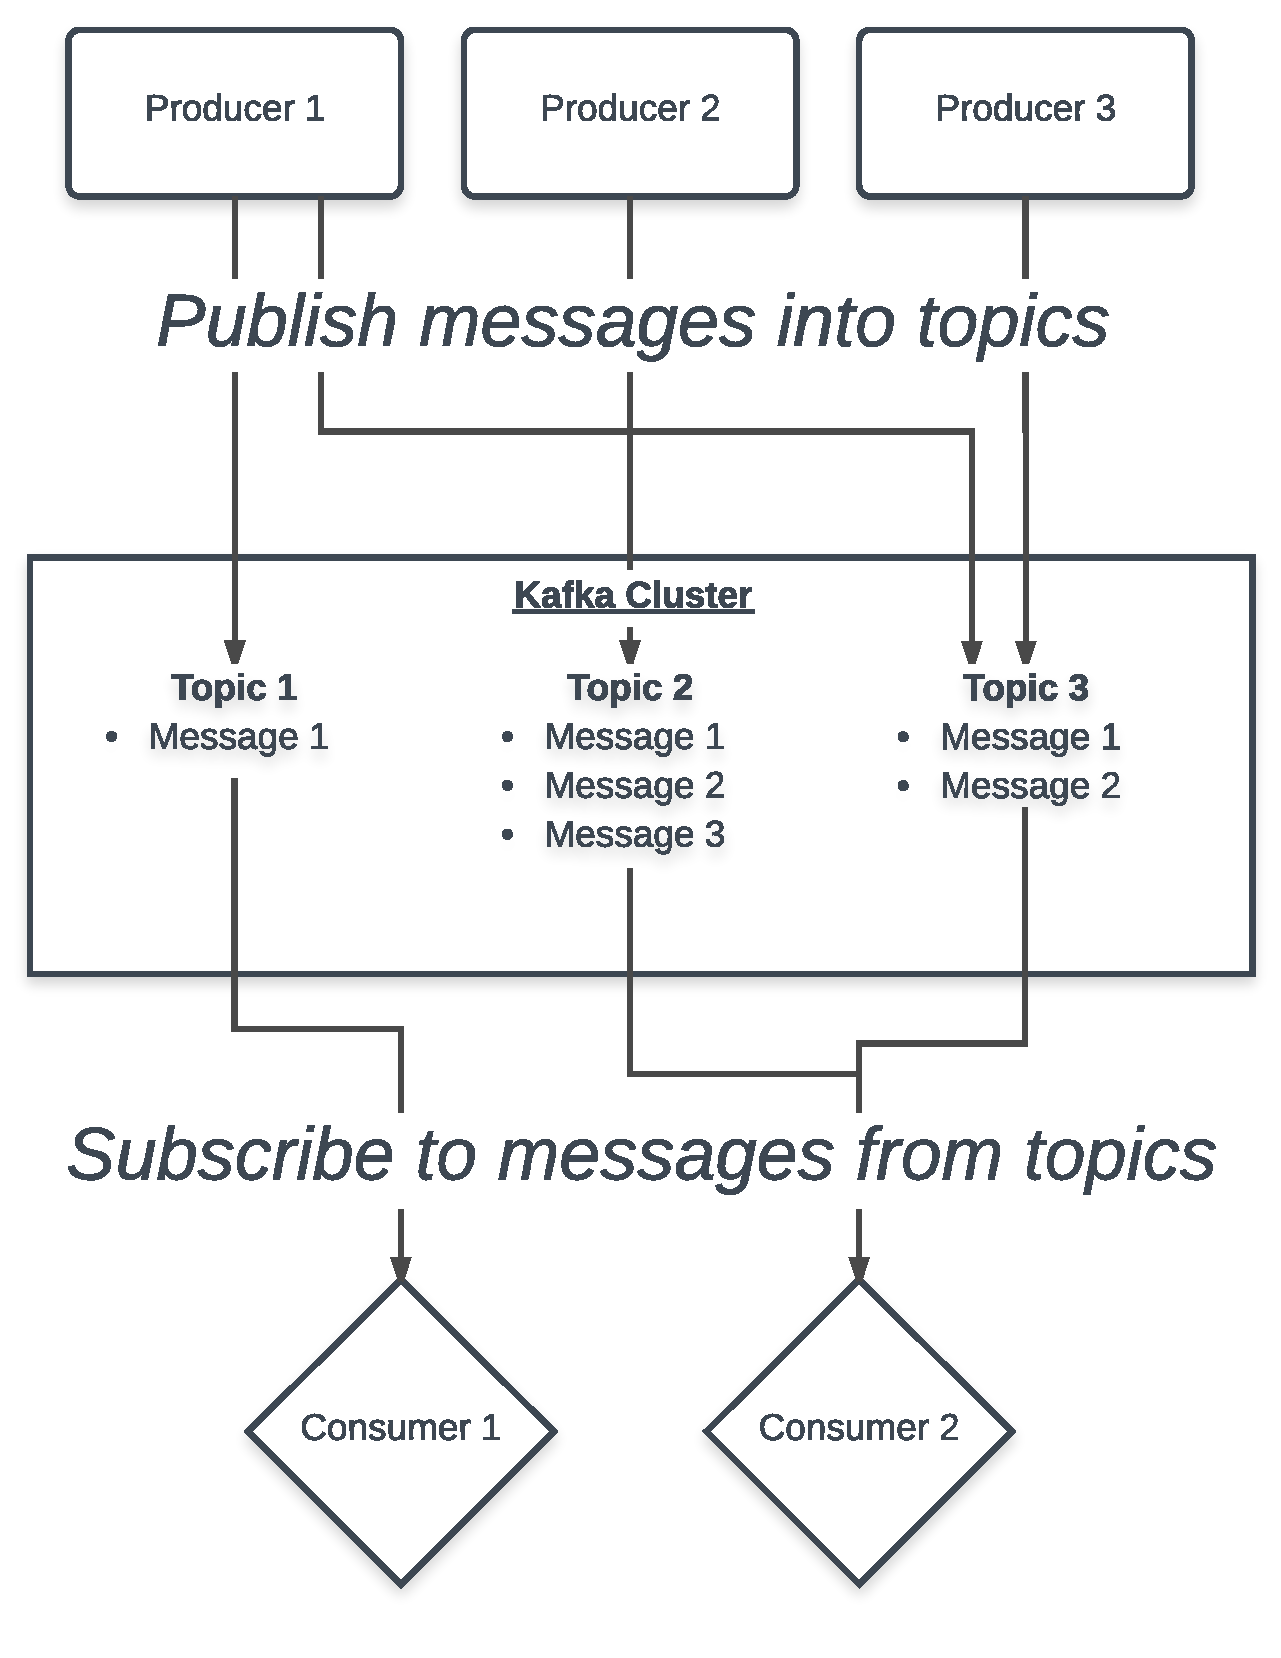
\includegraphics[width=\textwidth]{../figures/kafka.pdf}
\end{figure}

The system, as seen in~\ref{fig:kafka}, scales vertically, enabling high throughput and redundance.

% Figure and Code example
\subsection{Spark}
\label{subsec:spark}

Important: Spark plugs into Kafka very nicely as a consumer

Explaining Spark and how it was used
\begin{itemize}
    \item
    Spark offers some good data analysis functions (showing an example that shows Spark's strengths) % TODO (maybe show wordcount code here)
    \item
    Comparing the DataFrame-based and of the RDD-based API of Spark
    \item
    But Spark's real strength lies in the fact any library can be used on the execution node, which is why I use other libraries quite liberally for the best workflow (See chapters \ref{sentimentanalysis} and \ref{ch:topicModeling})
    \item
    The Factory pattern was used often because of how python handles scopes
    \item
    Why it makes sense and what is transmitted to the exec nodes in the end
    \item
    First using a queueStream, but it doesn’t work in the python API, switched to starting a Kafka stream (Kafka just has to be running somewhere, on connect the stream is connected to the Kafka broker and the sparkjob is immediately submitted with the session id as a parameter)
\end{itemize}

\subsection{NLTK}
\label{subsec:nltk}

Explaining the NLTK and how it was used, but not yet talking about the sentiment analysis algorithms it offers.
Those are introduced and explained in detail in their chapters.

\section{Project Structure}
\label{sec:projectStructure}


Using the DS cookie cutter, except the streaming folder is one under source because it is used by data to collect training data and by visualization for the dashboard.
Generally a modular approach that can be easily expanded with further analysis/monitoring beyond the LDA/Sentiment Analysis with Naive Bayes combination has been build.


\section{Architecture}
\label{sec:architecture}

Explaining the choice of architecture with some figures.
% TODO architecture diagram from the book
About 2 pages total introducing the technologies.


In our case, we only have one execution node, but Kafka and Spark are designed such that there should not be a problem
\pagebreak[2]